\section{L07-Cicli a gas}
\subsection{Cicli termodinamici a gas}
Vedremo molte formule e molti passaggi che però non è essenziale imparare benissimo. Queste formule semplificate saranno solo \textbf{valide per cicli ideali}, quindi nel momento in cui si analizza un ciclo reale non valgono più. Ciò che sarà applicabile anche nei casi reali sono le definizioni che mostreremo.\newline
\newline
Nei cicli termodinamici a gas faremo sempre l'\textbf{ipotesi} semplificativa \textbf{di gas perfetti} (anche se non è sempre propriamente valido).\newline
\newline
Esistono numerosi cicli:
\begin{itemize}
    \item Ciclo di Carnot (ciclo puramente teorico, irrealizzabile nella realtà);
    \item Ciclo Joule-Brayton (tipico degli aerei);
    \item Ciclo Otto (tipico ciclo che utilizza benzina, quindi automobili, tosaerba, etc);
    \item Ciclo Diesel (tipico per le applicazioni a potenze elevate);
    \item Ciclo Stirling (importante a livello storico);
    \item Ciclo Ericsson;
\end{itemize}
\subsubsection{Proprietà dei cicli simmetrici}
Un ciclo termodinamico è tipicamente rappresentato da $4$ \textbf{politropiche}, uguali a due a due, per cui prende il nome di ciclo \textbf{simmetrico}. Non sempre questa ipotesi di simmetria è presente.
\begin{center}
    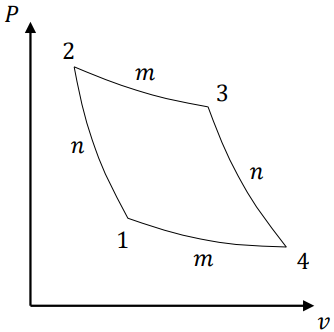
\includegraphics[height=3cm]{../L07/img1.PNG}
\end{center}
Nel caso di \textbf{ciclo ideale} (politropiche senza irreversibilità, cioè trasformazioni internamente reversibili) e ipotesi di \textbf{gas ideale}:
\[
    \begin{matrix}
        v_1v_3 = v_2v_4\\
        P_1P_3 = P_2P_4\\
        T_1T_3 = T_2T_4
    \end{matrix}
\]
(Queste formule derivano dalla scrittura delle politropiche di ogni trasformazione e utilizzando l'equazione di stato dei gas ideali e facendo alcuni passaggi e calcoli).\newline
\newline
La maggior parte dei cicli che andremo a vedere sono principalmente utilizzati per macchina motrici (che producono lavoro). Più avanti vedremo esempi di cicli inversi che verranno usati per macchine operatrici.\newline
\newline
Fino ad ora per le macchine termodinamiche abbiamo parlato dei serbatori di calore a temperatura calda e fredda e del serbatoio di lavoro, ora ci focaliziamo sulla macchina ciclica che opera su questi serbatoi.\newline
\newline
Il termine $S_{irr}$ che abbiamo nel bilancio entropico può essere scomposto in $S_{irr,est}$, cioè le irreveribilità esterne (legate ai serbatoi e agli scambi), e $S_{irr, int}$, cioè le irreversibilità interne della macchina ciclica (irreversibilità delle trasformazioni). Nel caso ideale non avremo irreversibilità esterne, quindi nessuna irreversibilità nei serbatoi e negli scambi con la macchina ciclica. Se le tr
\subsection{Ciclo di Carnot}
Il \textbf{ciclo di Carnot} è un \textbf{ciclo teorico} composto da $4$ trasformazioni tutte internamente reversibili e l'unica combinazioni di trasformazioni politropiche che soddisfano queste richieste sono \textbf{due isoentropiche e due isoterme}.
\begin{center}
    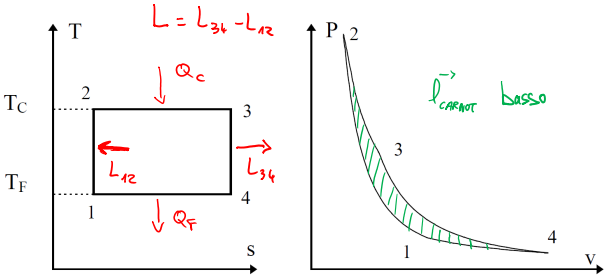
\includegraphics[height=4cm]{../L07/img2.PNG}
\end{center}
In (2-3) avviene lo scambio di calore con il serbatoio di calore superiore, in (4-1) avviene lo scambio di calore con il serbatoio di calore inferiore. Queste due sono le trasformazioni isoterme. Invece lungo le isoentropiche (1-2) e (3-4) non abbiamo scambi di calore, ma solo di lavoro, le isoentropiche sono adiabatiche reversibili. Il lavoro totale uscente dal ciclo (il lavoro prodotto) sarà calcolabile come $L = L_{34} - L_{12}$. \newline
\newline
Questo ciclo rappresenta il ciclo ideale che si cerca di ottenere per una macchina per avere il rendimento massimo.\newline
\newline
Guardando il diagramma P-V vediamo che l'area interna al ciclo (che rappresenta il lavoro specifico) è molto ridotto. Il lavoro specifico del ciclo di Carnot è molto basso, nonostante il rendimento sia massimo. Questo vuol dire che per avere una certa potenza dobbiamo avere un impianto di dimensioni notevoli.\newline
\newline
\subsubsection{Rendimento del ciclo}:
\[
    \eta = \frac{L}{Q_C} = 1-\frac{Q_F}{Q_C} = 1- \frac{T_1}{T_3}    
\]
\ \newline
\newline
\textbf{Possibili fonti di irreversibilità per una macchina termodinamica}:
\begin{itemize}
    \item \textbf{Irreversibilità esterna ($T_{min} > T_F$ e $T_{max} < T_C$)}:\newline
    Ricordiamo che $T_1 = T_4 = T_{min}$ e $T_2 = T_3 = T_{max}$.
    \begin{center}
        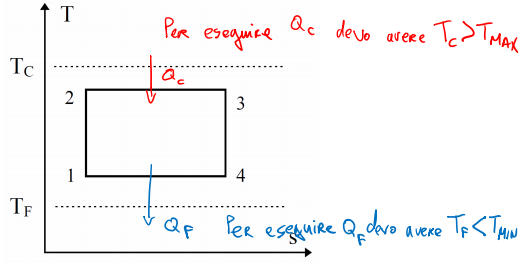
\includegraphics[height=3cm]{../L07/img3.PNG}
    \end{center}
    Tipico caso di irreversibiltà esterna è il fatto che le temperature dei serbatoi non coincidano con le temperature delle trasformazioni.
    \[
        \eta_{rev} = 1-\frac{T_F}{T_C} > \eta_{ciclo} = 1- \frac{T_1}{T_3} = 1- \frac{T_{min}}{T_{max}}
    \]
    Bilancio entropico su tutta la macchina termica (reale):
    \[
        -\frac{Q_C}{T_C} + \frac{Q_F}{T_F} = S_{irr}
    \]
    Per il ciclo di Carnot vale:
    \[
        \frac{Q_C}{T_3} = \frac{Q_F}{T_1} = \Delta S
    \]
    Che risolta rispettoa $Q_F$:
    \[
        Q_C\left(\frac{1}{T_F} \frac{T_1}{T_3} - \frac{1}{T_C}\right) = S_{irr}
    \]
    \[
        Q_C \left(\frac{T_C T_1 - T_F T_3}{T_3T_CT_F}\right) = S_{irr, est} > 0
    \]
    \item \textbf{Irreversibilità interna ($s_1 > s_2$ e $s_3 < s_4$)}:
    \item \begin{center}
        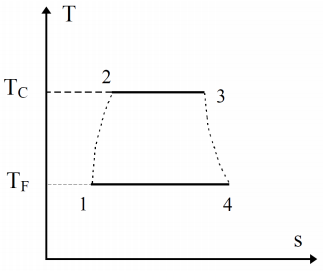
\includegraphics[height=3cm]{../L07/img4.PNG}
    \end{center}
    In questo caso non abbiamo più isoentropiche, ma trasformazioni reali, per cui si ha un incremento di entropia.\newline
    Bilancio entropico su tutta la macchina termica (reale):
    \[
        - \frac{Q_C}{T_C} + \frac{Q_F}{T_F} = S_{irr}
    \]
    per cui:
    \[
        \frac{Q_C}{T_C} = S_3 - S_2
    \]
    \[
        \frac{Q_F}{T_F} = S_4 - S_1
    \]
    e sostitendo:
    \[
        S_2-S_3 +S_4 -S_1 = S_{irr, int} > 0
    \]
\end{itemize}
Nel caso in cui si abbiano entrambe le irreversibilità, le due componenti si sommano.
\subsection{Ciclo di Joule-Bryton}
\textbf{Caso simmetrico costituitio da due isoentropiche e due isobare}:\newline
Abbiamo detto che il ciclo di Carnot è ideale, per cui non ha applicazioni reali interessanti. Una miglioria che si può fare è quella di considerare trasdormazioni isobare per lo scambio termico. Così facendo si ha un forte incremento della potenza prodotta (area interna al ciclo nel grafico P-V):
\begin{center}
    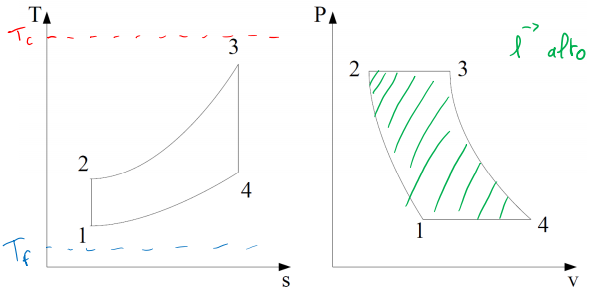
\includegraphics[height=4cm]{../L07/img5.PNG}
\end{center}
Struttura della macchina ciclica per il ciclo di Brayton:
\begin{center}
    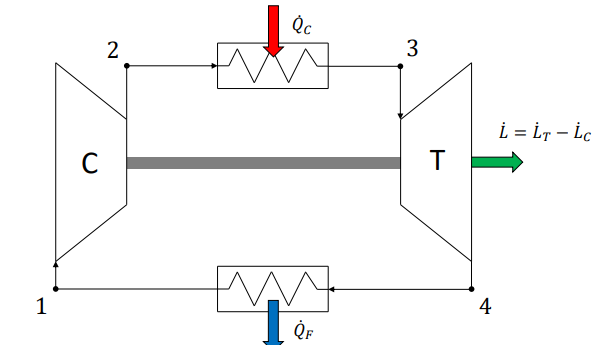
\includegraphics[height=5cm]{../L07/img6.PNG}
\end{center}
dove \newline
$C$: è un compressore che esegue la prima isoentropica;\newline
In alto: uno scambiatore di calore che fa il suo scambio in maniera isobara;\newline
$T$: turbina a gas che esegue la seconda isoentropica;\newline
La barra grigia in centro: mostra che c'è un collegamento fra turbina e compressore, o meglio che turbina e compressore sono sullo stesso asse di rotazione e quindi c'è una trasmissione diretta di potenza fra la turbina e il compressore (una parte di lavoro generata dalla turbina è utilizzata per alimentare il compressore);\newline
In basso: un'altro scambiatore di calore isobaro.\newline
\newline
\subsubsection{Rendimento del ciclo J-B (gas perfetto, ciclo ideale simmetrico)}
Con l’ipotesi di gas perfetto, le equazioni di bilancio energetico per i due serbatoi
di calore sono:
\[
        \dot{Q}_C = \dot{m} (h_3-h_2) \;\;\;\;\;\;\;\;\;\; \dot{Q}_F = \dot{m}(h_4 -h_1)
\]
che con l'ipotesi dei gas perfetti diventa:
\[
    \dot{Q}_C = \dot{m} c_P(T_3-T_2) \;\;\;\;\;\;\;\;\;\; \dot{Q}_F = \dot{m}c_P (T_4-T_1)
\]
Il rendimento termodinamico del ciclo vale:
\[
    \eta_{J-B} = \frac{\dot{L}}{\dot{Q}_C} = 1 - \frac{\dot{Q}_F}{\dot{Q}_C} = 1- \frac{T_4-T_1}{T_3-T_2} = 1- \frac{T_1 \left(\frac{T_4}{T_1} - 1\right)}{T_2 \left(\frac{T_3}{T_2}-1\right)} = 1- \frac{T_1}{T_2}
\]
Inserendo il bilancio di entropia fra 1 e 2 per i gas perfetti:
\[
    \Delta s_{12} = c_P ln \frac{T_2}{T_1}- R^* ln \frac{P_2}{P_1}
\]
\[
    \left(\frac{T_2}{T_1}\right)^{c_P} = \left(\frac{P_2}{P_1}\right)^{R^*}
\]
\[
    \left(\frac{T_2}{T_1}\right) = \left(\frac{P_2}{P_1}\right)^{\frac{R^*}{c_P}} = r_P^{\frac{R^*}{c_P}} = r_P^{\frac{k-1}{k}}
\]
dove $r_P$ è il \textbf{rapporto di compressione} ($\frac{P_2}{P_1}$, che è $\frac{P_{max}}{P_{min}}$) per cui il rendimento è riscrivibile come
\[
    \eta_{J-B} = 1- \frac{1}{r_P^{\frac{k-1}{k}}}
\]
dove $k$ è l'indice della politropica e vale $k = \frac{c_P}{c_V} = costante$.\newline
\newline
Il rendimento del ciclo Joule-Brayton è funzione del solo rapporto di compressione e presenta un minimo (rendimento nullo) quando la pressione $P_2$ tende alla pressione $P_1$ e quindi
\[
    r_{P,min} = 1
\]
mentre ha un valore massimo quando $T_2$ tende a $T_3$, e pertanto
\[
    r_{P,max} = \left(\frac{T_3}{T_1}\right)^{\frac{k}{k-1}}
\]
\subsubsection{Lavoro specifico del ciclo J-B (gas perfetto, ciclo ideale simmetrico)}
Possiamo fare lo stesso ragionamento anche per il lavoro specifico, cioè il lavoro prodotto.\newline
Anche il lavoro specifico utile del ciclo Joule-Brayton ideale è funzione del solo rapporto di compressione
\[
    l = l_T-l_C = c_P (T_3-T_4) - c_P(T_2-T_1)
\]
\[
    l = c_P T_3 \left(1- \frac{T_4}{T_3}\right) - c_P T_1 \left(\frac{T_2}{T_1} - 1\right)
\]
\[
    l = c_P T_3 \left(1- \frac{1}{r_P^{\frac{k-1}{k}}}\right) - c_P T_1 \left(r_P^{\frac{k-1}{k}}-1\right)
\]
Per cui si ha il massimo lavoro specifico in corrispondenza del rapporto di compressione:
\[
    r_{P,opt} = \left(\frac{T_3}{T_1}\right)^{\frac{k}{2(k-1)}} = \sqrt{r_P,max}
\]
Ricordando poi che in una turbina isoentropica
\[
    \frac{T_3}{T_4} = \left(\frac{P_3}{P_4}\right)^{\frac{R^*}{c_P}} = \left(\frac{P_3}{P_4}\right)^\frac{k-1}{k}
\]
E inserendo in questa espressione al posto di $\frac{P_3}{P_4}$ (pari a $\frac{P_2}{P_1}$) il valore di $r_{P,opt}$ e sfruttando le proprietà dei cicli simmetrici, si ottiene:
\[
    T_4 = T_2 = \sqrt{T_1 T_3}
\]
cioè il lavoro specifico è massimo nel ciclo in cui la temperatura di fine espansione coincide con quella di fine compressione.\newline
\newline
Questo risultato ci dice che per un ciclo in cui non vale $T_4 = T_2$ (cioè in cui non si ha un lavoro ottimale), per migliorare il ciclo bisogna cercare di avvicinare il più possibile questi valori di temperature.
\begin{center}
    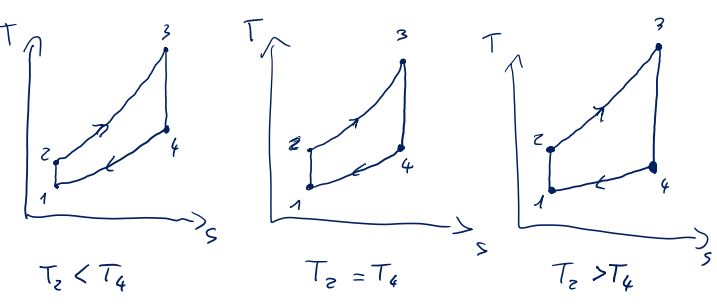
\includegraphics[height=4cm]{../L07/img7.PNG}
\end{center}
L'immagine centrale rappresenta il caso ottimale. Le immagini laterali no, a sinistra l'uscita della turbina è più calda rispetto all'uscita del compressore, a destra l'uscita della turbina è più fredda dell'uscita del compressore.
\subsubsection{Ciclo Joule-Brayton con rigenerazione}
Una delle soluzioni che può portare a un migliroamento del rendimento e del lavoro specifico prodotto che si può applicare al caso $T_2<T_4$, ovvero in cui la temperatura in uscita dalla turbina è maggiore della temperatura in uscita dal compressore.
\begin{center}
    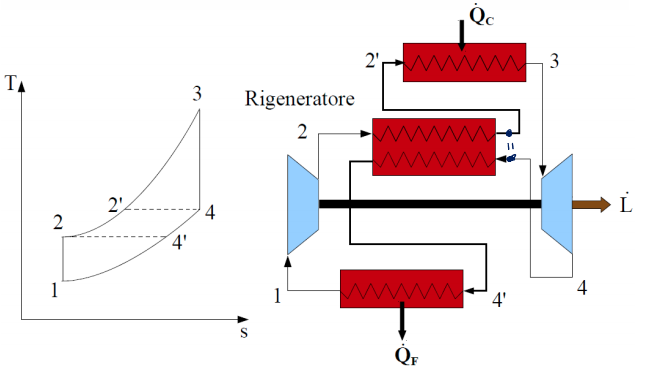
\includegraphics[height=6cm]{../L07/img8.PNG}
\end{center}
La corrente calda in uscita dalla turbina in eccesso viene sfruttata per innalzare la temperatura in uscita dal compressore.\newline
\newline
Per fare questo preriscaldamento durante il riscaldamento (2-3) possiamo utilizzare un rigeneratore (che è uno scambiatore) in modo da trasferire calore fra ciò che esce dalla turbina verso quello che esce dal compressore e quindi recuperare questa energia. Sfruttando questa energia in più il compressore dovrà solo eseguire una trasformazione (2'-3) e non più (2-3) e così si ha un risparmio sulla spesa.\newline
\newline
\subsubsection{Rendimento del ciclo rigenerato ideale}
Per ciclo rigenerato \textbf{ideale} si intende che $T_{2'} = T_4$ (si è recuperata tutta l'energia), che si lavora con gas perfetti e che il ciclo è ideale e simmetrico.
\[
    \eta_{rig} = \frac{\dot{L}}{\dot{Q}_C} = \frac{\dot{L}_T - \dot{L}_C}{\dot{Q}_C} = \frac{(T_3-T_4)-(T_2-T_1)}{(T_3-T_4)} = 1- \frac{T_2-T_1}{T_3-T_4}
\]
\[
    \eta_{rig} = 1- \frac{T_2}{T_3} = 1- \frac{T_2 T_1}{T_3T_1}
\]
\[
    \eta_{rig} = 1- \frac{T_1}{T_3}r_P^{\frac{k-1}{k}}
\]
In una rigenerazione ideale si ha che $T_{2'}=T_4$, mentre in una reale si ha che $T_{2'} < T_4$ (è necessario un salto termico per effettuare lo scambio).